\section{Timing Compartments}

This section introduces a new architecture abstraction, named timing compartment.
We first discuss the type of timing channels that the timing compartment is designed
to prevent. Then, we define the timing compartment, describe our threat model,
and discuss application scenarios that the timing compartments can enable.


\subsection{Taxonomy of Timing Channels}

%    \begin{figure}
%        \begin{center}
%            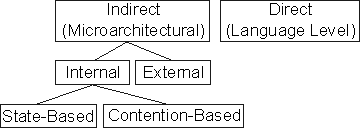
\includegraphics[width=2.2in]{figs/taxonomy.pdf}
%            \caption{The taxonomy of timing channels}
%            \label{fig:taxonomy}
%        \end{center}
%    \end{figure}

A timing channel represents a security vulnerability where the timing of events
depend on confidential information. An adversary can use timing channels as
side channels to learn secrets such as cryptographic keys or passwords or as
covert channels to intentionally bypass restrictions on communications.

%Figure~\ref{fig:taxonomy} summarizes the taxonomy of timing channels. \emph{Direct} or 
%language level timing channels can be identified by examining the source code 
%\cite{mitigation3}. A password checking algorithm that stops as soon as an 
%incorrect character is found causes a direct timing channel that leaks 
%information about the correct password. In contrast, \emph{indirect} or 
%microarchitectural timing channels cannot be identified in the source code 
%since they depend on hardware level behavior \cite{mitigation3}. Conventional 
%caches cause an indirect timing channel whenever the probability of a cache hit 
%depends on secret data. Programming language techniques have been developed to 
%address language level timing channels 
%\cite{timesens,mitigation1,mitigation2,mitigation3}. It is possible to reduce 
%the information leaked by some microarchitectural timing channels at the 
%language level \cite{mitigation3}. However, eliminating all leakage caused by 
%microarchitectural timing channels is difficult without hardware support.
%%%% More precise, wordier version:
%  However, efficiently providing strict timing-sensitive noninterference in 
%  the presence microarchitectural timing channels without the support of 
%  hardware is a hard problem.

Timing channels can be categorized into {\em external} and {\em internal} 
\cite{mitigation3}. 
External timing channels exist when the timing of a program's event that
can be observed externally leak information on data that the program processes. 
For example, a password checking program that sequentially compares strings
and stops on the first incorrect character leaks where a mismatch is.
As another example, Bernstein's attack~\cite{bernstein} exploits data-dependent
timing variations in a popular implementation of an AES encryption.
%Adversaries can carry out external timing channel attacks even without sharing 
%hardware with a victim program. 
Because the external timing channels happen when a program's operation differs
depending on a secret, language-level techniques have been developed to
mitigate them \cite{timesens,mitigation1,mitigation2,mitigation3}. 

%further divided into internal or 
%external timing channels. \emph{External} timing channels are not caused by 
%interference, and are exploited by an adversary that directly measures the 
%timing of the victim's actions. External timing channels can be exploited by an 
%adversary that does not share hardware with the victim. Bernstein's 
%attack~\cite{bernstein} exploits an external timing channel in popular 
%implementations of AES (such as OpenSSL). The external timing channel exists 
%because the cache access pattern both affects the overall execution time of the 
%AES implementation and depends on the secret key. The adversary carries out the 
%attack without sharing any hardware by directly measuring the response times of 
%the victim machine.
%%%%% The long explanation
% The adversary uses a copy of the same AES implementation as the victim to 
% time the encryption of a number inputs with a known key on the adversary's 
% local machine. Then, the adversary makes requests to the victim machine using 
% the same inputs and times how long the victim machine takes to encrypt the 
% inputs with an unknown key. In both cases, the execution time depends on the 
% cache access pattern which depends on the key. The adversary can use the 
% timing information gathered with the known and unknown keys to learn the 
% secret AES key.

Internal timing channels exist when one program's timing depends on another
program that shares the same hardware due to interference. In this case,
an adversary can exploit the timing channel by measuring the timing of its
own events even without directly observing a victim program.
For example, Percival~\cite{percival} showed an internal timing channel
through a shared cache where an attack program can extract an AES key
by measuring its own cache access time, which reflects a victim program's
cache accesses that depend on the key.



\subsection{Definition of Timing Compartments}

A timing compartment is a new architecture abstraction that allows software to
explicitly control {\em internal timing channels} that exist in shared systems. 
The ability to control timing channels, combined with a traditional access
control mechanism such as virtual memory, enables complete software isolation
because the timing channel is the only form of side/covert channels that can be
exploited in software without physical attacks.

From the software perspective, a timing compartment consists of one or more software 
entities such as threads, processes, and virtual machines. 
Then, software can express a policy that specifies which timing channels among
timing compartments are allowed or not. In general, the policy can take a form
of a lattice model, which defines ordering between security levels \cite{denning}.
This lattice model is quite expressive and widely used for information flow control. 
For example, the lattice may restrict timing channels only in one direction 
from $\mathtt{TC1}$ to $\mathtt{TC2}$ ($\mathtt{TC2} \leq \mathtt{TC1}$).
The lattice may disallow any timing channel between two compartments by making
them incomparable ($\mathtt{TC_1} \nleq \mathtt{TC_2}$, $\mathtt{TC_2} \nleq \mathtt{TC_1}$).

%Here, a software 
%entitiy is some system abstraction (such as processes or threads in a single OS 
%system or virtual machines in a virtualization based system) that execute 
%software and have an owner. Intuitively, a single timing compartment contains 
%only software entities that trust each other explicitly (such as all the VMs on 
%a machine owned by the same user) or implicitly (all the VMs that do not want 
%to pay for protection), and leakage within a timing compartment is safe.

Similar to other architecture abstractions such as virtual memory, the
timing compartments need to be implemented as a combination of hardware-software
mechanisms. The underlying hardware must provide mechanisms to distinguish
events from different timing compartments and control timing interference 
in shared resources.
Then, a trusted software component needs to manage the hardware mechanisms 
at run-time. We call this trusted software as timing compartment manager (TCM).

%To enforce the policy, a trusted software component called the timing 
%compartment manager (TCM) confines software entities into TCs. The TCM then 
%informs the hardware of the TCs and policy. At runtime, the TCM tags software 
%requests for hardware to indicate the TC of the software entity that made the 
%request. The hardware then enforces the policy by controlling how requests from 
%different TCs share resources.

The timing compartments allows software to explicitly control timing channels
among groups of software entities, but does not enforce any restrictions within
each compartment. We believe that handling timing channels separately from
traditional isolation abstractions such as processes and virtual machines is essential
to allow efficient system designs. Because timing channel protection is more expensive
than traditional access control, a designer should be able to pay the overhead
of timing control only when truly necessary.

%Timing compartments only address timing channels; they do not control 
%information flow through explicit channels. Handling these concerns separately 
%allows for more flexibility in the overall system design.  When designing a 
%secure system, implementors must consider how the cost required to carry out a 
%particular attack compares with other attacks, the potential damage that could 
%be caused by an attack, and the cost and performance impact of implementing the 
%security mechanisms needed to stop it. This enables timing compartments to 
%provide timing channel protection only to software entities that need it.

\subsection{Threat Model}

%Goal
The goal of the timing compartment is to enable complete software isolation
on shared hardware, comparable to having separate hardware for each.
%Assumptions
In that sense, we assume that a target system has multiple cores with shared
resources such as caches, on-chip interconnect, and off-chip memory that can
be used by multiple programs concurrently. The system can also be time multiplexed.
%The multicore system of interest consists of hardware resources that are
%concurrently shared by multiple software entities. It is possible for software 
%entities to be time multiplexed on the same core (e.g.  by context switching 
%VMs), but the system does not allow software entities to execute concurrently 
%on the same core (e.g. through simultaneous multithreading). 
We also assume that there exists a trusted software layer such as an OS or a hypervisor,
which provides conventional software isolation for explicit communication channels.
The timing compartment manager (TCM) is assumed to be a part of this trusted software.

%Attacks we handle.
%However, these approaches to isolate software do not address timing channels 
%that leverage shared hardware. To guarantee total isolation, internal timing 
%channels must also be eliminated. We eliminate all internal microarchitectural 
%timing channels including state and state-based timing channels. 
%This includes 
%all timing channels caused by concurrently shared resources as well as timing 
%channels in hardware that is shared through time multiplexing (e.g. by context 
%switching).

The timing compartment aims to eliminate {\em internal} timing channels through
interference in shared microarchitecture resources. In particular, the goal is
to prevent both unintentional (side channels) and intentional (covert channels)
information leaks.
However, external timing
channels, which exist even with dedicated hardware, are not prevented by the
timing compartments. If necessary, the external timing channels can be controlled 
in software. 
Similarly, timing channels through I/O devices are not considered in this study
because their accesses can be controlled in software.
Finally, we not consider physical attacks on the system such as
physical side-channel attacks through power consumption or electromagnetic emission. 

%Attacks we don't handle.
%Since our goal is to address vulnerabilities 
%caused by hardware sharing,
%timing channels that are external to the hardware are not addressed.
%Any timing channels that are external to the hardware in this system would also 
%be present if the software entities executed on separate hardware. If 
%necessary, external timing channels can be controlled in software. Similarly, 
%we do not address language level timing channels since these may also be 
%addressed in software.  Lastly, we do not consider physical attacks and assume 
%that the adversary does not have physical access.


\subsection{Application Scenarios}

The ability to control internal timing channels can significantly increase a level of
assurance in a number of applications where distrusting entities share a
physical system. Here, we briefly discuss representative applications.

\subsubsection{Bring Your Own Device (BYOD)}

As mobile devices such as smartphones and tablets are becoming widely used, 
companies and government organizations are starting to allow employees to
use their own devices to access corporate data. This trend is often called
Bring Your Own Device (BYOD). However, there is a major concern that such a
mixed use can lead to a leak of confidential data through personal emails or
downloaded applications. Today's BYOD solutions such as Samsung Knox uses
software containers or virtualization to separate the two environments:
personal and work. Yet, these solutions cannot prevent information leaks
through internal timing channels.

\begin{figure}
    \begin{center}
        \includegraphics[width=1.51in]{figs/app_byod.pdf}
        \caption{A BYOD example.}
        \label{fig:app_byod}
    \end{center}
\end{figure}

The timing compartment enables a strong isolation guarantee in the BYOD
scenario. For example, consider the solution based on virtualization as 
shown in Figure~\ref{app:byod}. In this case, the virtual machines for
work and personal use can be assigned to two different timing compartment:
$TC_{work}$ and $TC_{pers}$. Then, the lattice can be set so that no
information can flow from $TC_{work}$ to $TC_{pers}$.
Note that the BYOD application only requires two timing compartments even
though a system may have many cores and run many applications.

\subsubsection{High-Assurance Cloud Computing}

In cloud computing such as Amazon EC2, virtual machines (VMs) from multiple
distrusting clients often share physical machines. 
%A cloud provider 
%co-locates many VMs on a single machine to increase its utilization,
%and tenants often have little control over where their VMs run. 
For example, a tenant may share hardware with competitors or attackers that 
want to extract sensitive data. Today's virtualization technologies restrict 
explicit communication channels among virtual machines, but cannot control 
internal timing channels. In fact, recent studies have shown that timing channels
can be exploited in commercial clouds to extract secrets such as 
a password \cite{FIXME}.
For some clients, timing channels may not be a major concern. Yet, for enterprise
or government clients who require high assurance, this security threat makes
public cloud computing not an option. 

\begin{figure}
    \begin{center}
        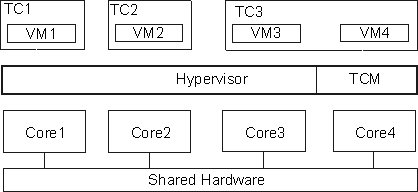
\includegraphics[width=2.79in]{figs/cloud_tcs.pdf}
        \caption{A cloud computing example. VM1 
        and VM2 have high security requirements, but VM3 and VM4 do not.}
        \label{fig:cloud_tcs}
    \end{center}
\end{figure}

The timing compartment can enable high assurance cloud computing by ensuring that
there cannot be unintended information leak among virtual machines.
Figure~\ref{fig:cloud_tcs} shows an example with four virtual machines (VMs).
%that have different security requirements. 
VM1 and VM2 require a strong isolation guarantee and distrust other VMs.
VM3 and VM4 run low-security applications that are not concerned with timing channels
but require high performance. The figure shows that three timing compartments can
be used to meet the security requirements in this example.
VM1 and VM2 are placed in their own timing compartments $TC1$ and $TC2$, but 
VM3 and VM4 are grouped in $TC3$. The lattice can be set so that VM1 and VM2
cannot leak information to any VM but no constraint is put on VM3 and VM4:
$TC3 \leq TC1, TC3 \leq TC2, TC1 \nleq T2, TC2 \nleq TC1$.
%TC3 preceeds both TC1 and TC2 implying timing channel leakage from VM3 or VM4 to 
%any other VM is not controlled. However, VM1 and VM2 cannot leak information to 
%VM3 or VM4. Additionally, VM1 and VM2 cannot leak information to each other 
%since TC1 and TC2 are incomparable. This meets the security requirements of VM1 
%and VM2 since both are totally isolated from the other VMs through timing 
%channels. Since VM3 and VM4 share a timing compartment, they can share 
%resources normally and incur minimal performance overheads.


\subsubsection{Untrusted Software} 

The ability to completely eliminate timing channels enables timing compartments
to be used to contain information even when software is potentially malicious.
For example, today's smartphone users often rely on many third party applications
that cannot be fully trusted to manage private or sensitive data. A system may
sandbox an untrusted application and restrict its communication channels
when it accesses sensitive data. However, today's access control mechanisms cannot
prevent the untrusted application from leaking information to another unrestricted
application through internal timing channels. The timing compartment can be added 
to provide a complete sandbox. 
In the cloud computing context, the same timing channel protection can be used
by a cloud provider to sandbox a third-party web services that cannot be fully trusted.

\subsubsection{Safety-Critical Systems}

In addition to protecting confidential data, the capability to control interference
in shared hardware can also be used to provide timing guarantees on safety-critical systems.
For example, hard real-time systems such as automotive controllers must meet
strict timing requirements. Unfortunately, today's multi-core processors provide
no timing guarantee when shared by multiple programs. The timing compartment can be
used to ensure that the timing of safety-critical components are not affected by
the rest of a system.

